%%%% compile with
%%% latexmk -auxdir=aux/ main.tex
\documentclass{irdbeamer}
\usepackage{tikz}
\usepackage{pgfplots}
\usepackage{animate}

\title{Sampling and overfitting}
\subtitle{AI for ecologists}
\author[Paul Tresson]{Paul Tresson}
\date{21/05/25} % or whatever the date you are presenting in is
% \institute[Institut de Recherche pour le Développement]{UMR AMAP}

%\copyrightnotice{Published by Institut de Recherche pour le Développement, with permission}

% %% to add a background image for the title slide, uncomment here
% \usebackgroundtemplate{
%   \tikz[overlay, remember picture] \node[at=(current page.center)] {
%     \includegraphics[width=\paperwidth,height=\paperheight]{example-image-a}
%   };
% }

\usepackage[
    backend=biber,
    style=authoryear-comp,
    maxcitenames=2, % max 2 authors before switching to et al.
    maxbibnames=4,
    uniquelist=false, % stays et al. when almost the same authors
    uniquename=false, % dose not bother when first name not written the same way everywhere
    date=year, % month does not appear in bibliography
    natbib=true, % use natbib synthax
    url=false, % remove url
    eprint=false % remove eprint
]{biblatex}

\addbibresource{refs.bib}

\let\oldcite=\cite                                                              
\renewcommand{\cite}[1]{\textcolor[rgb]{.5,.5,.7}{\oldcite{#1}}}
\let\oldcitep=\citep                                                              
\renewcommand{\citep}[1]{\textcolor[rgb]{.5,.5,.7}{\oldcitep{#1}}}

\begin{document}

\addlogo{logos/IRD_banner.png}
\addlogo{logos/AMAP_banner.png}
\addlogo{logos/CESAB.jpg}
\maketitle

\usebackgroundtemplate{}

\section{Introduction}

\begin{frame}{What do we want when modelling ?}
    \begin{itemize}
        \item<1-> Understand things
        \item<2-> \textbf{Predict things}
    \end{itemize}
\end{frame}

\begin{frame}{What do we want when modelling ?}
    
    \Large{
    \textit{
        "All models are wrong, but some are useful"
        }
    }

    \hfill George E. P. Box
\end{frame}

\begin{frame}{What do we want when modelling ?}
    \begin{itemize}
        \item \textbf{Robustness}: Useful when mistakes
        \item \textbf{Generalization}: Useful applied elsewhere
    \end{itemize}
\end{frame}

\section{Overfitting}

\begin{frame}{What is overfitting}
    \centering
    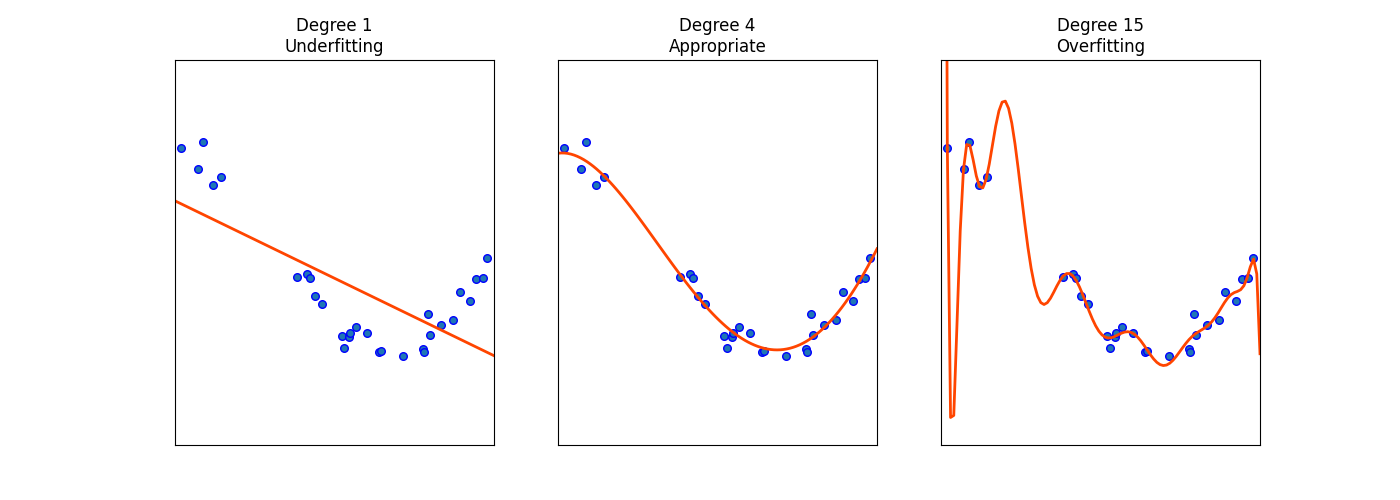
\includegraphics[width = .8\textwidth]{./figs/overfitting-overview.png}
    \nonumbernote{\tiny adapted from scikit-learn docs}
\end{frame}

\begin{frame}{Common tools and intuitions - Train/Test loss}
    \begin{columns}
        \begin{column}{.5\linewidth}
    \centering
    \vspace{1cm}
    \includegraphics<1>[width = .8\textwidth]{./figs/plot/overfitting1.png}%
    \includegraphics<2>[width = .8\textwidth]{./figs/plot/overfitting2.png}%
    \includegraphics<3>[width = .8\textwidth]{./figs/plot/overfitting3.png}%
    \includegraphics<4>[width = .8\textwidth]{./figs/plot/overfitting4.png}%
    \includegraphics<5>[width = .8\textwidth]{./figs/plot/overfitting5.png}%
    \includegraphics<6>[width = .8\textwidth]{./figs/plot/overfitting6.png}%
    \includegraphics<7>[width = .8\textwidth]{./figs/plot/overfitting7.png}%
    \includegraphics<8>[width = .8\textwidth]{./figs/plot/overfitting8.png}%
    \includegraphics<9>[width = .8\textwidth]{./figs/plot/overfitting9.png}%
        \end{column}
        \begin{column}{.5\linewidth}
    \centering
    \includegraphics<1>[width = .8\textwidth]{./figs/plot/train_test_loss-1.png}%
    \includegraphics<2>[width = .8\textwidth]{./figs/plot/train_test_loss-2.png}%
    \includegraphics<3>[width = .8\textwidth]{./figs/plot/train_test_loss-3.png}%
    \includegraphics<4>[width = .8\textwidth]{./figs/plot/train_test_loss-4.png}%
    \includegraphics<5>[width = .8\textwidth]{./figs/plot/train_test_loss-5.png}%
    \includegraphics<6>[width = .8\textwidth]{./figs/plot/train_test_loss-6.png}%
    \includegraphics<7>[width = .8\textwidth]{./figs/plot/train_test_loss-7.png}%
    \includegraphics<8>[width = .8\textwidth]{./figs/plot/train_test_loss-8.png}%
    \includegraphics<9>[width = .8\textwidth]{./figs/plot/train_test_loss-9.png}%
        \end{column}
    \end{columns}
\end{frame}

\begin{frame}{Common tools and intuitions - Train/Test loss}
    \begin{figure}
        \centering
        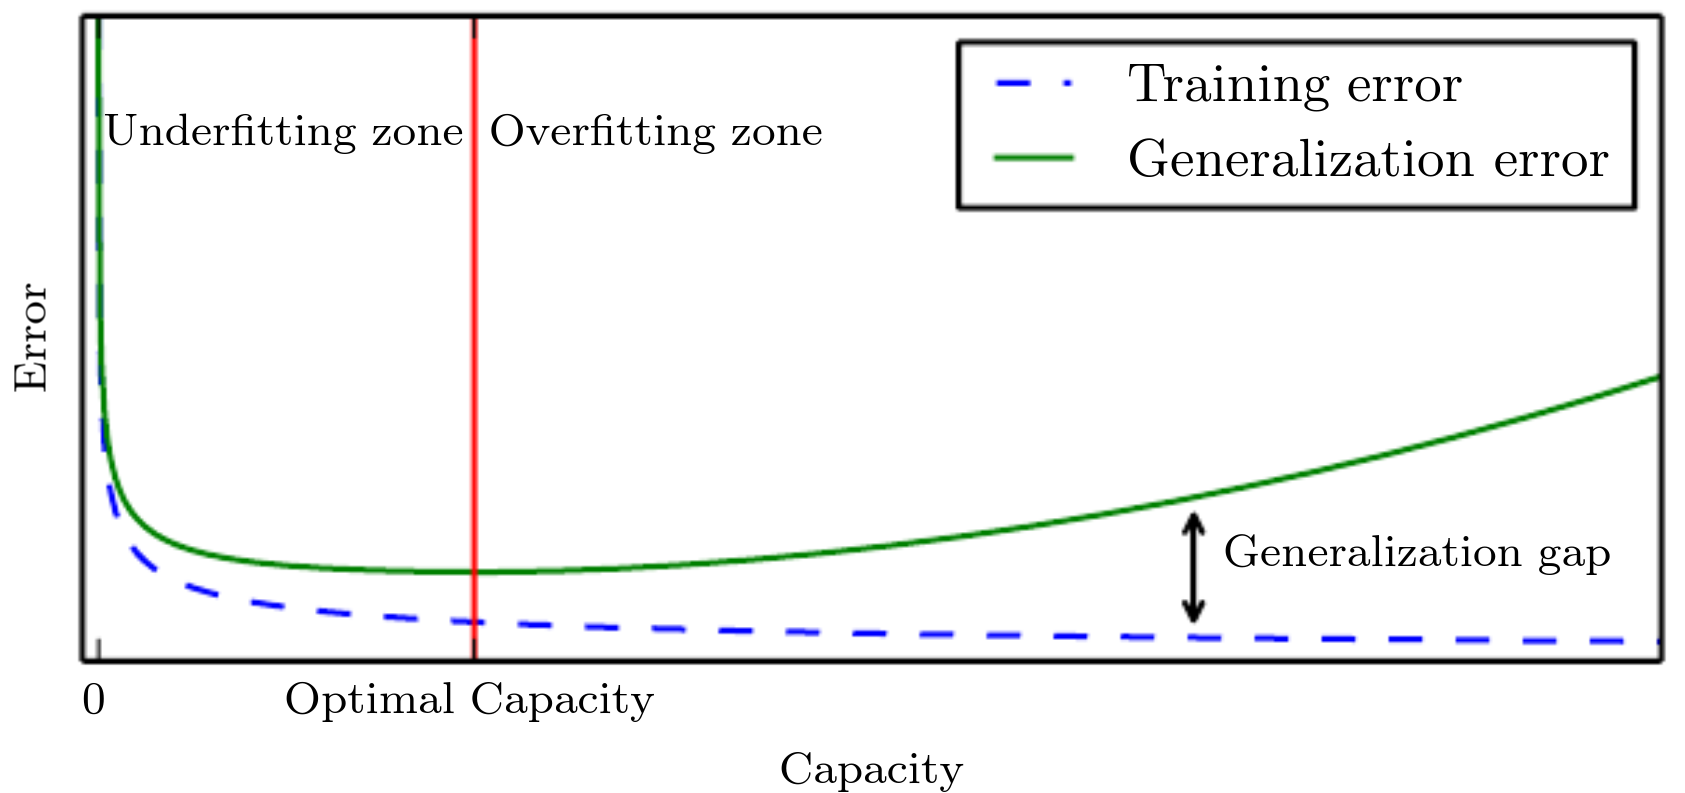
\includegraphics[width = .8\textwidth]{./figs/goodfellow.png}
        \caption{\tiny Figure from \cite{goodfellow2016deep}}
    \end{figure}
\end{frame}

\begin{frame}{Common tools and intuitions - AIC/BIC}
    \begin{center}
    \textbf{Akaike information criterion (AIC)}

    \textbf{Bayesian information criterion (BIC)}

        Is the model parameter efficient ?
    \end{center}
\end{frame}

\begin{frame}{Common tools and intuitions - Biases}
    \begin{figure}
        \centering
        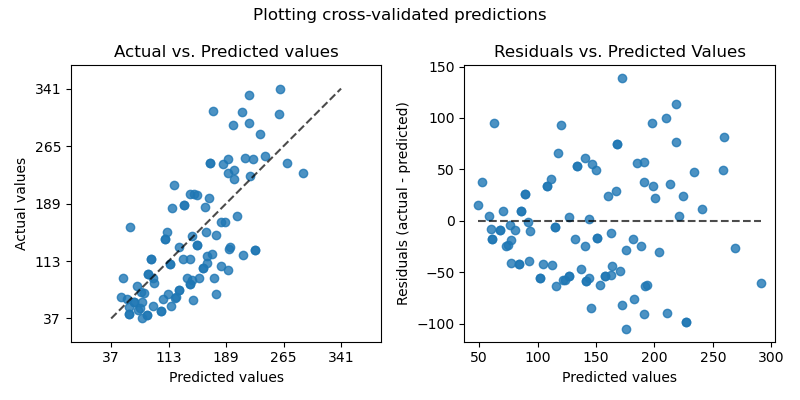
\includegraphics[width = .8\textwidth]{./figs/residuals.png}
    \end{figure}
    \nonumbernote{\tiny from scikit-learn docs}
\end{frame}

\begin{frame}{And in Machine(/Deep) Learning ??}
    \centering
    How many parameters to have\\
    \textbf{Shrek learning botany starting from random noise ?}
\end{frame}

\begin{frame}{And in Machine(/Deep) Learning ??}
    \centering
        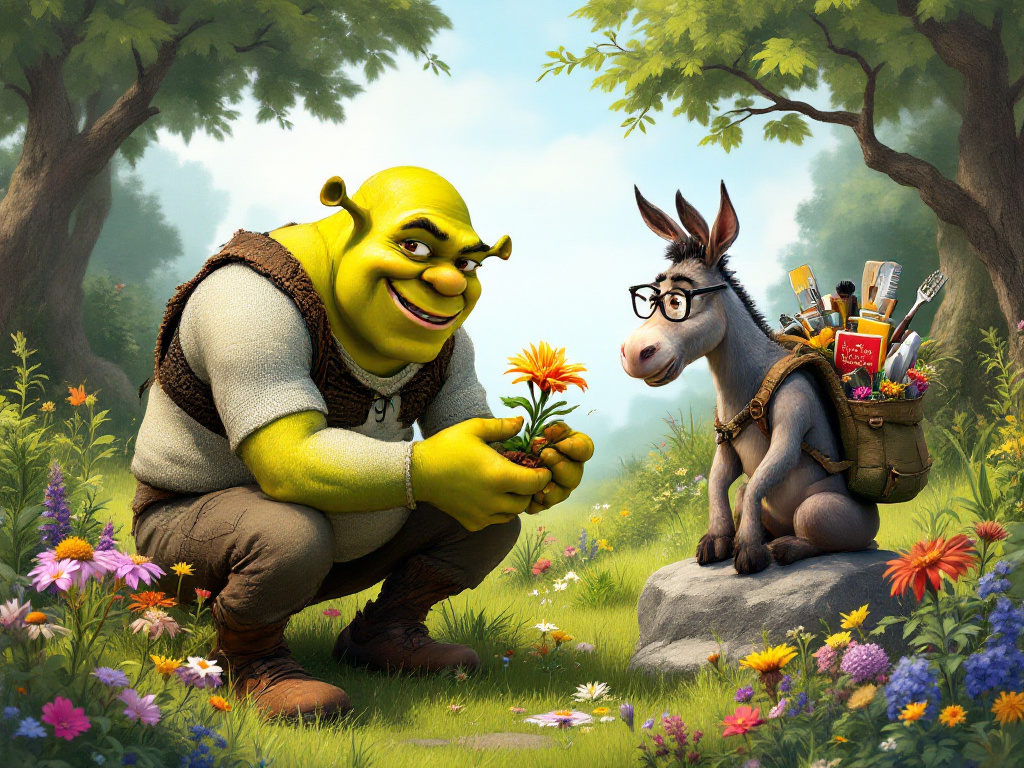
\includegraphics[width = .5\textwidth]{./figs/shrek.jpg}

        $\approx 2.5B$ ?
\end{frame}

\begin{frame}{Root Causes}
    \centering
    \only<1->{\textbf{Too many parameters}}

    \only<2->{\textbf{Too little training data}}

    \only<3>{\textbf{(bad) training data}}
\end{frame}


\section{Illustrated examples in Ecology}

\begin{frame}[t]{Contraints in ecology}
    \only<1->{Data from the real world is noisy,}%
    \only<2->{ unbalanced,}%
    \only<3->{ hard to collect,}%
    \only<4->{ hard to interpret.}%

            \centering
    \includegraphics<1>[width=.8\textwidth]{./figs/bouamir.png}%
    \includegraphics<2>[width=.7\textwidth]{./figs/plantnet_longtail.png}%
    % \only<2>{\tiny \\Distribution of species represented in plantnet dataset}
    \includegraphics<3>[width=.3\textwidth]{./figs/climbing.png}%
    \includegraphics<4>[width=.3\textwidth]{./figs/recapcha.png}%
    \includegraphics<5>[width=.3\textwidth]{./figs/recapcha_plantnet.png}%
    \includegraphics<6>[width=.3\textwidth]{./figs/recapcha_pheidole.png}%
\end{frame}

\begin{frame}{}
    \centering
    \includegraphics<1>[width=.5\textwidth]{./figs/schemas/train.png}%
    \includegraphics<2>[width=.5\textwidth]{./figs/schemas/good_fit.png}%
    \includegraphics<3>[width=.5\textwidth]{./figs/schemas/good_fit_test.png}%
    \includegraphics<4>[width=.5\textwidth]{./figs/schemas/bad_fit.png}%

    \only<1>{Train set}%
    \only<2>{\small A good fitted model}%
    \only<3>{Test set}%
    \only<4>{\footnotesize An overfitted model}%
\end{frame}

\begin{frame}{Biases in the train set}
    \begin{columns}
        \begin{column}{.5\linewidth}
            \centering
    \includegraphics<1-2>[width=.9\textwidth]{./figs/monstera-plantnet.png}%
    \includegraphics<3>[width=.5\textwidth]{./figs/monstera-wild.jpg}%
        \end{column}
        \begin{column}{.5\linewidth}
            \centering
    \includegraphics<1>[width=.8\textwidth]{./figs/schemas/train.png}%
    \includegraphics<2>[width=.8\textwidth]{./figs/schemas/good_fit.png}%
    \includegraphics<3>[width=.8\textwidth]{./figs/schemas/bad_test.png}%
        \end{column}
    \end{columns}
\end{frame}

\begin{frame}{Biases in the train set - autocorrelation}
    \begin{columns}
        \begin{column}{.5\linewidth}
            \centering
    \includegraphics<1>[width=.8\textwidth]{./figs/camera_trap_frames.png}%
    \includegraphics<2>[width=.8\textwidth]{./figs/camera_trap_frames1.png}%
    \includegraphics<3->[width=.8\textwidth]{./figs/camera_trap_frames2.png}%
        \end{column}
        \begin{column}{.5\linewidth}
            \centering
    \includegraphics<2>[width=.8\textwidth]{./figs/schemas/train.png}%
    \includegraphics<3>[width=.8\textwidth]{./figs/schemas/autocorr_test.png}%
    \includegraphics<4>[width=.8\textwidth]{./figs/schemas/autocorr.png}%
        \end{column}
    \end{columns}
\end{frame}

% \begin{frame}{Unbalanced data}
%     \begin{columns}
%         \begin{column}{.5\linewidth}
%             \centering
%     \includegraphics<1->[width=.8\textwidth]{./figs/plantnet_longtail.png}%
%         \end{column}
%         \begin{column}{.5\linewidth}
%             \centering
%     \includegraphics<1>[width=.8\textwidth]{./figs/schemas/unbalanced.png}%
%     \includegraphics<2>[width=.8\textwidth]{./figs/schemas/unb_tight.png}%
%     \includegraphics<3>[width=.8\textwidth]{./figs/schemas/unb_tight_test_unb.png}%
%     \includegraphics<4>[width=.8\textwidth]{./figs/schemas/test_unb_bad.png}%
%         \end{column}
%     \end{columns}
% \end{frame}

\begin{frame}{Unbalanced data}
            \centering
    \includegraphics<1>[width=.4\textwidth]{./figs/schemas/unbalanced.png}%
    \includegraphics<2>[width=.4\textwidth]{./figs/schemas/unb_tight.png}%
    \includegraphics<3>[width=.4\textwidth]{./figs/schemas/unb_tight_test_unb.png}%
    \includegraphics<4>[width=.4\textwidth]{./figs/schemas/test_unb_bad.png}%
\end{frame}

\begin{frame}{Deal with unbalanced data}
    \begin{columns}
        \begin{column}{.5\linewidth}
            \begin{itemize}
                \item<1-> Oversample ?
                \item<4-> Undersample/saturate ?
                \item<7-> Adapt loss ?
            \end{itemize}
        \end{column}
        \begin{column}{.5\linewidth}
            \centering
    \includegraphics<1>[width=.8\textwidth]{./figs/schemas/oversampled.png}%
    \includegraphics<2>[width=.8\textwidth]{./figs/schemas/oversampled_fit.png}%
    \includegraphics<3>[width=.8\textwidth]{./figs/schemas/fp.png}%
    \includegraphics<4>[width=.8\textwidth]{./figs/schemas/undersample.png}%
    \includegraphics<5>[width=.8\textwidth]{./figs/schemas/undersample_fit.png}%
    \includegraphics<6>[width=.8\textwidth]{./figs/schemas/fn.png}%
    \includegraphics<7>[width=.8\textwidth]{./figs/schemas/adapt_loss.png}%
        \end{column}
    \end{columns}
\end{frame}

\begin{frame}{Deal with lack of data}
    \begin{columns}
        \begin{column}{.5\linewidth}
            \begin{itemize}
                \item<1-> Data augmentation
                \item<3-> Pretrained model
                \item<4> \textbf{... collect more data}
            \end{itemize}
        \end{column}
        \begin{column}{.5\linewidth}
            \centering
    \includegraphics<1>[width=.8\textwidth]{./figs/schemas/train.png}%
    \includegraphics<2>[width=.8\textwidth]{./figs/schemas/data_aug.png}%
    \includegraphics<3>[width=.8\textwidth]{./figs/schemas/pretrained.png}%
        \end{column}
    \end{columns}
\end{frame}

\begin{frame}{Play with your model}
    \begin{columns}
        \begin{column}{.5\linewidth}
            \begin{itemize}
                \item Dropout
                \item Pruning
                \item Ablation studies
                \item Ensembles
            \end{itemize}
        \end{column}
        \begin{column}{.5\linewidth}
            \begin{figure}
            \centering
    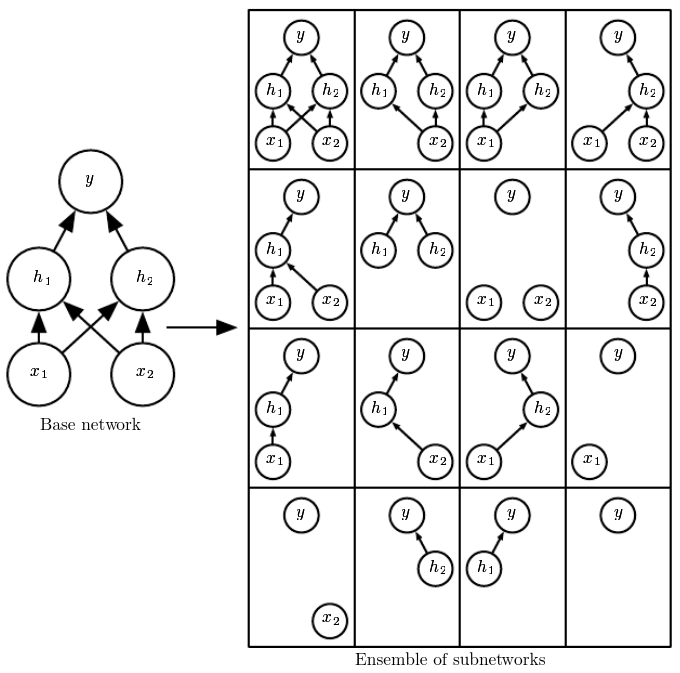
\includegraphics[width=.7\textwidth]{./figs/dropout.png}%
                \caption{\tiny Figure from \cite{goodfellow2016deep}}
            \end{figure}
        \end{column}
    \end{columns}
\end{frame}

\begin{frame}{}
    \centering
    \textbf{Need to be very carefull on how to evaluate}
\end{frame}

\section{How to sample and evaluate ?}

\begin{frame}{Random split ?}
    \begin{center}
    \textcolor{black}{"random split training validation 80/20"}
    \end{center}

    \pause
    
        \centering
        \vspace{-0.5cm}
            \fbox{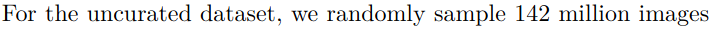
\includegraphics[width=.7\paperwidth,]{./figs/random_sampling.png}}

            \cite{oquab2023dinov2}
    
    \pause
    Works for huge DL papers, maybe not for you
\end{frame}

\begin{frame}{Cross-validation}
    \centering
    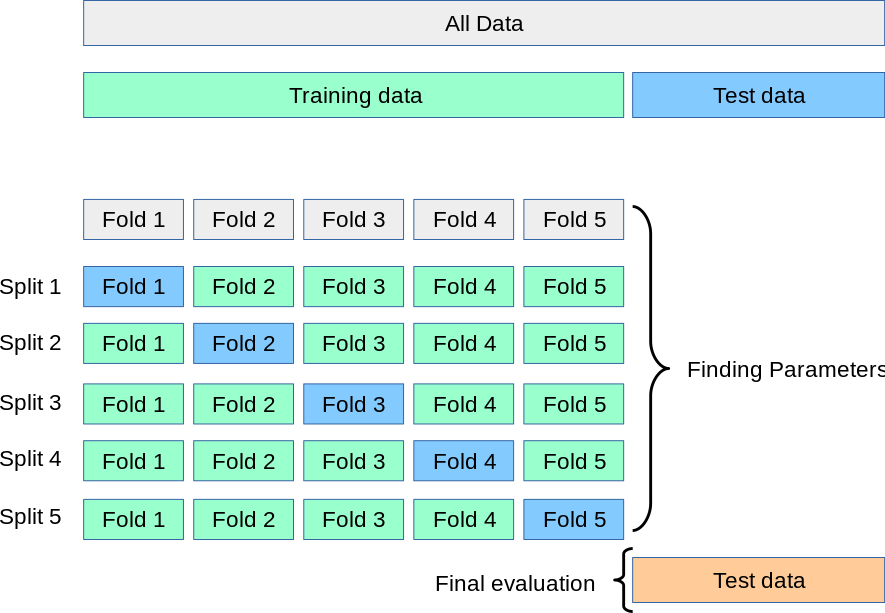
\includegraphics[width=.5\textwidth]{./figs/cross_validation.png}
    \nonumbernote{\tiny Figure from scikit-learn docs}
\end{frame}

\begin{frame}{Cross-validation}
    \centering
    \includegraphics<1>[width=.7\textwidth]{./figs/kfold.png}%
    \includegraphics<2>[width=.7\textwidth]{./figs/stratified_kfold.png}%
    \nonumbernote{\tiny Figure from scikit-learn docs}
\end{frame}

\begin{frame}{Case study : Spatial cross-validation}
    \begin{columns}
        \begin{column}{.5\linewidth}
            \centering
    \includegraphics<1-3>[width=.5\textwidth]{./figs/spatial/2022.png}%
    \includegraphics<4>[width=.5\textwidth]{./figs/spatial/2022_pleiades.png}%
        \end{column}
        \begin{column}{.5\linewidth}
            \centering
    \includegraphics<2>[width=.5\textwidth]{./figs/spatial/vit_dino_4cl.png}%
    \includegraphics<3->[width=.5\textwidth]{./figs/spatial/resnet_dino.png}%
        \end{column}
    \end{columns}
\end{frame}

\begin{frame}{Case study : Spatial cross-validation}
    \centering
    \includegraphics<1>[width=.5\textwidth]{./figs/spatial/ploton2020.png}%
    \includegraphics<2>[width=.5\textwidth]{./figs/spatial/ploton2020-result.png}%
    
    \tiny See. \cite{ploton2020spatial}
\end{frame}

\begin{frame}{Case study : Spatial cross-validation}
    \centering
    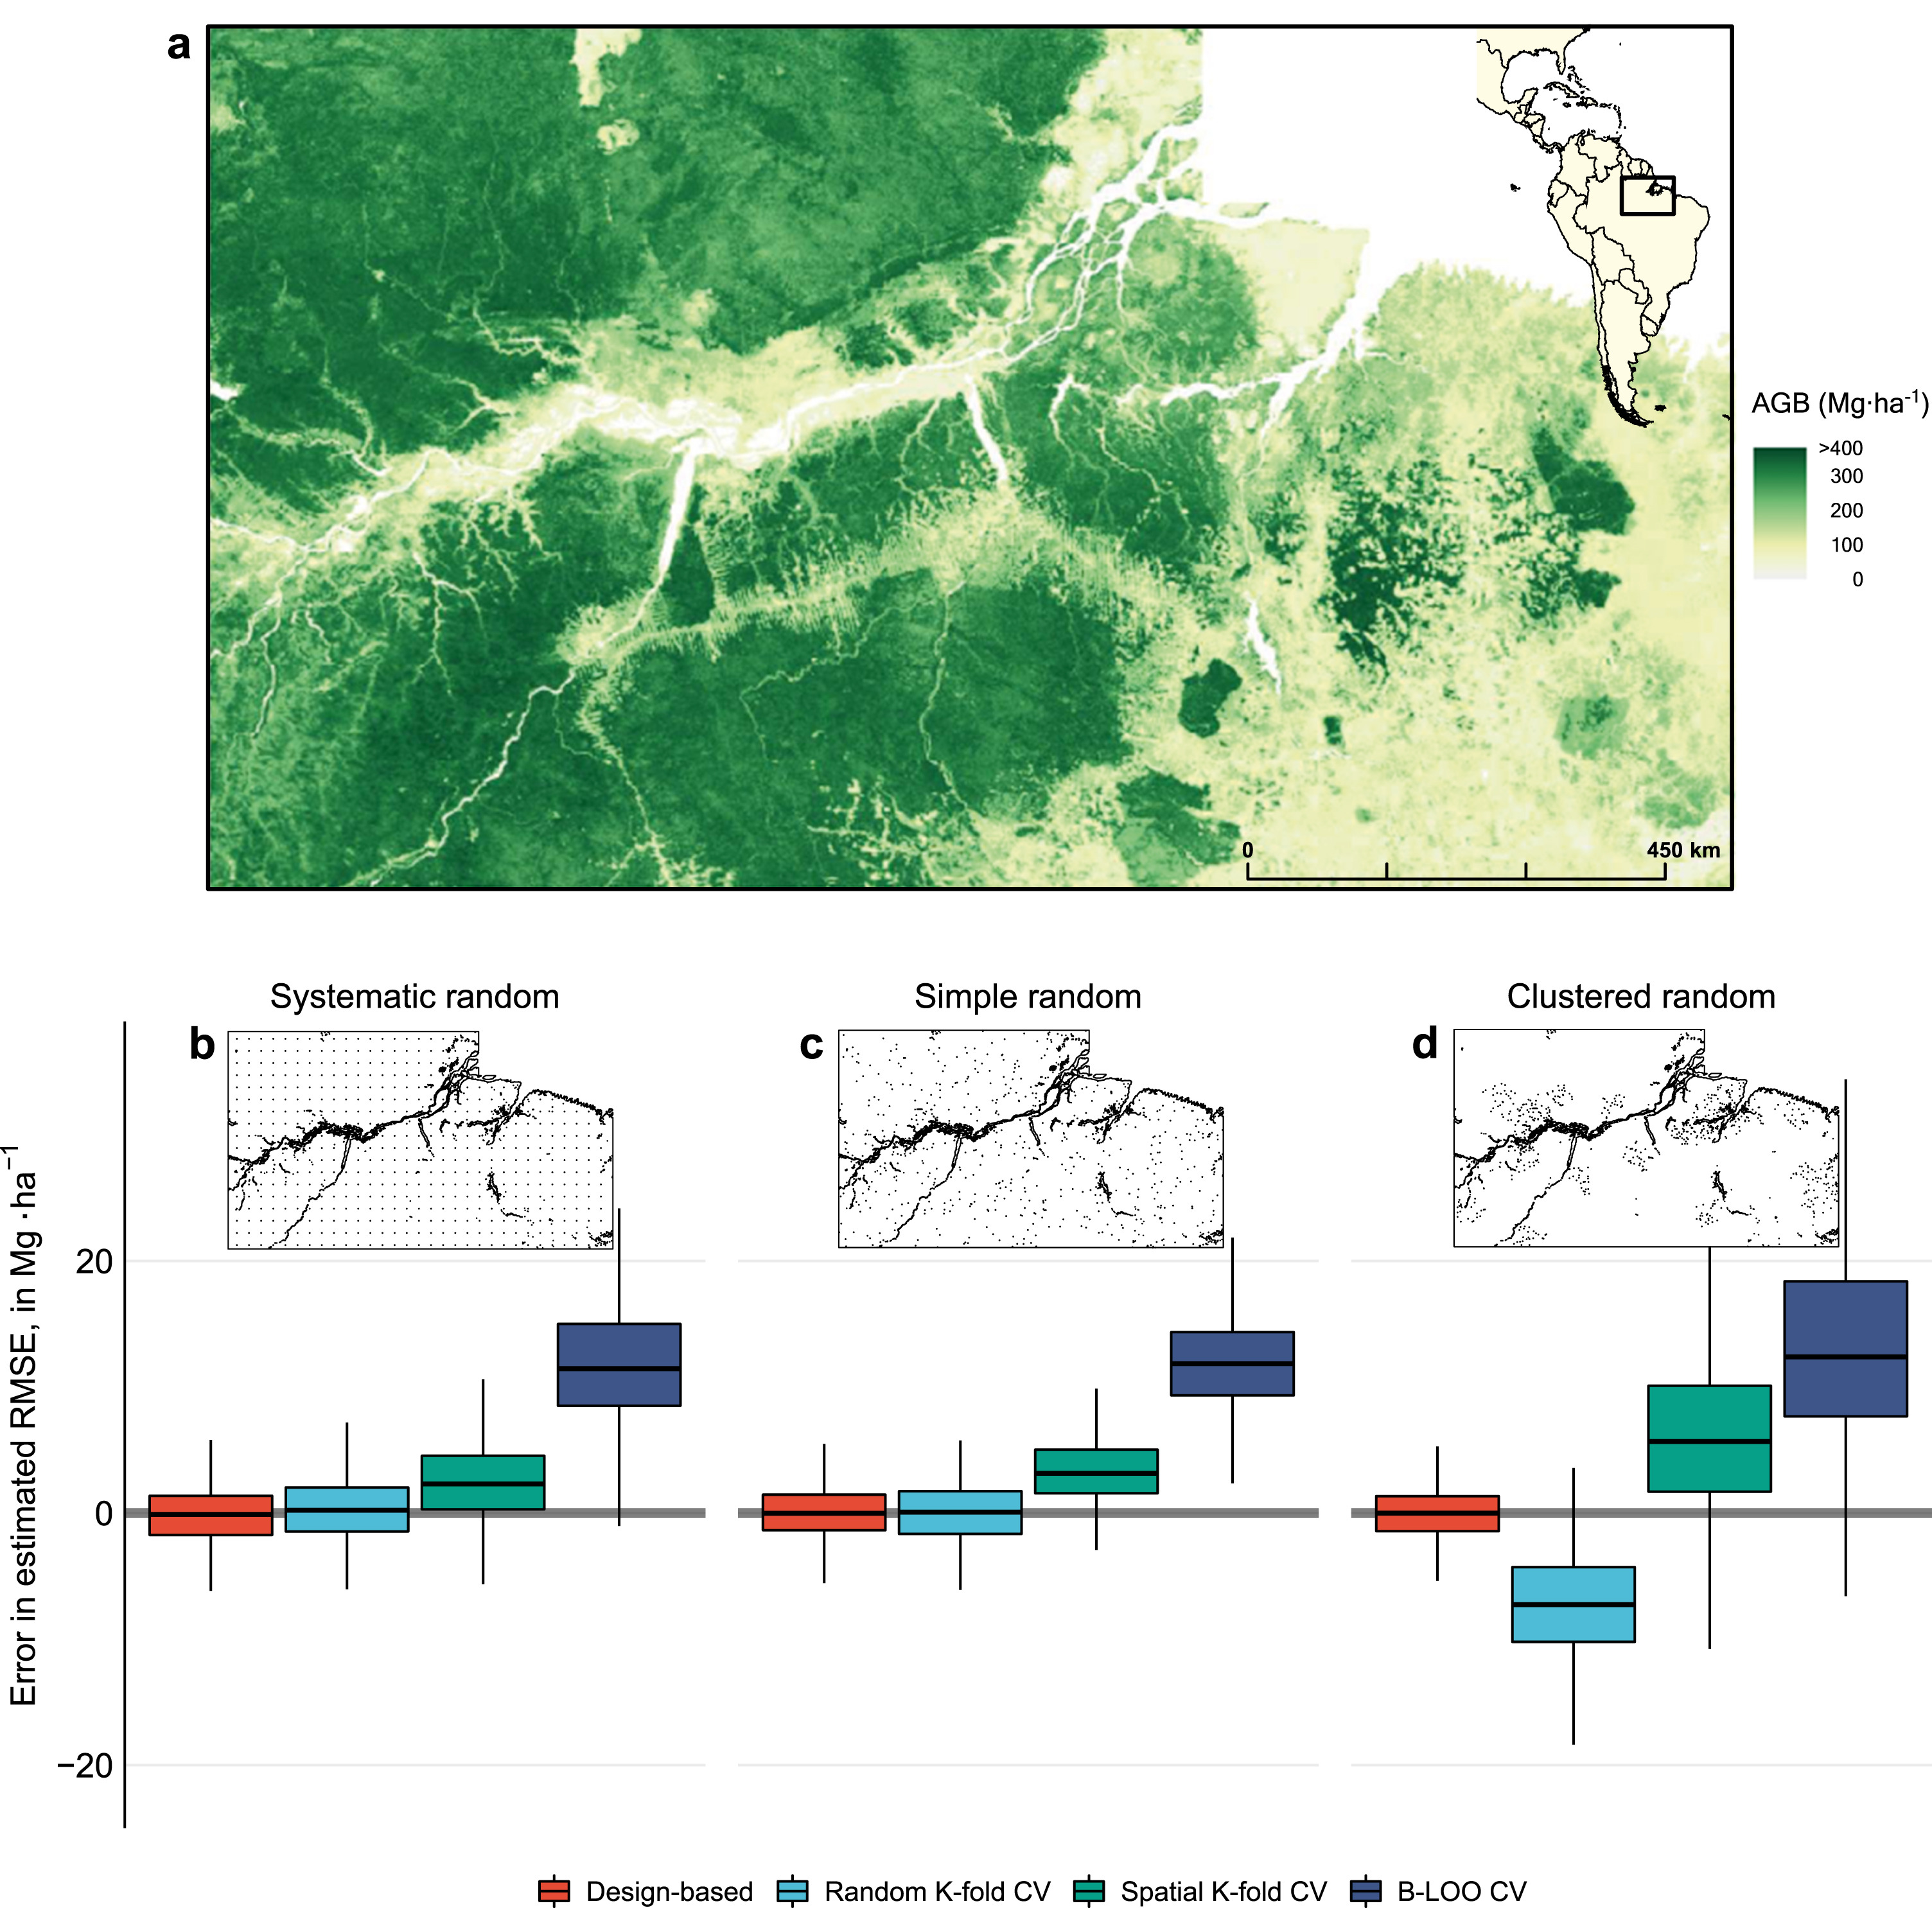
\includegraphics[width=.4\textwidth]{./figs/spatial/wadoux2021.jpg}%
    
    \tiny See. \cite{wadoux2021spatial}
\end{frame}

\begin{frame}{Case study : Aging models ?}
    \centering
    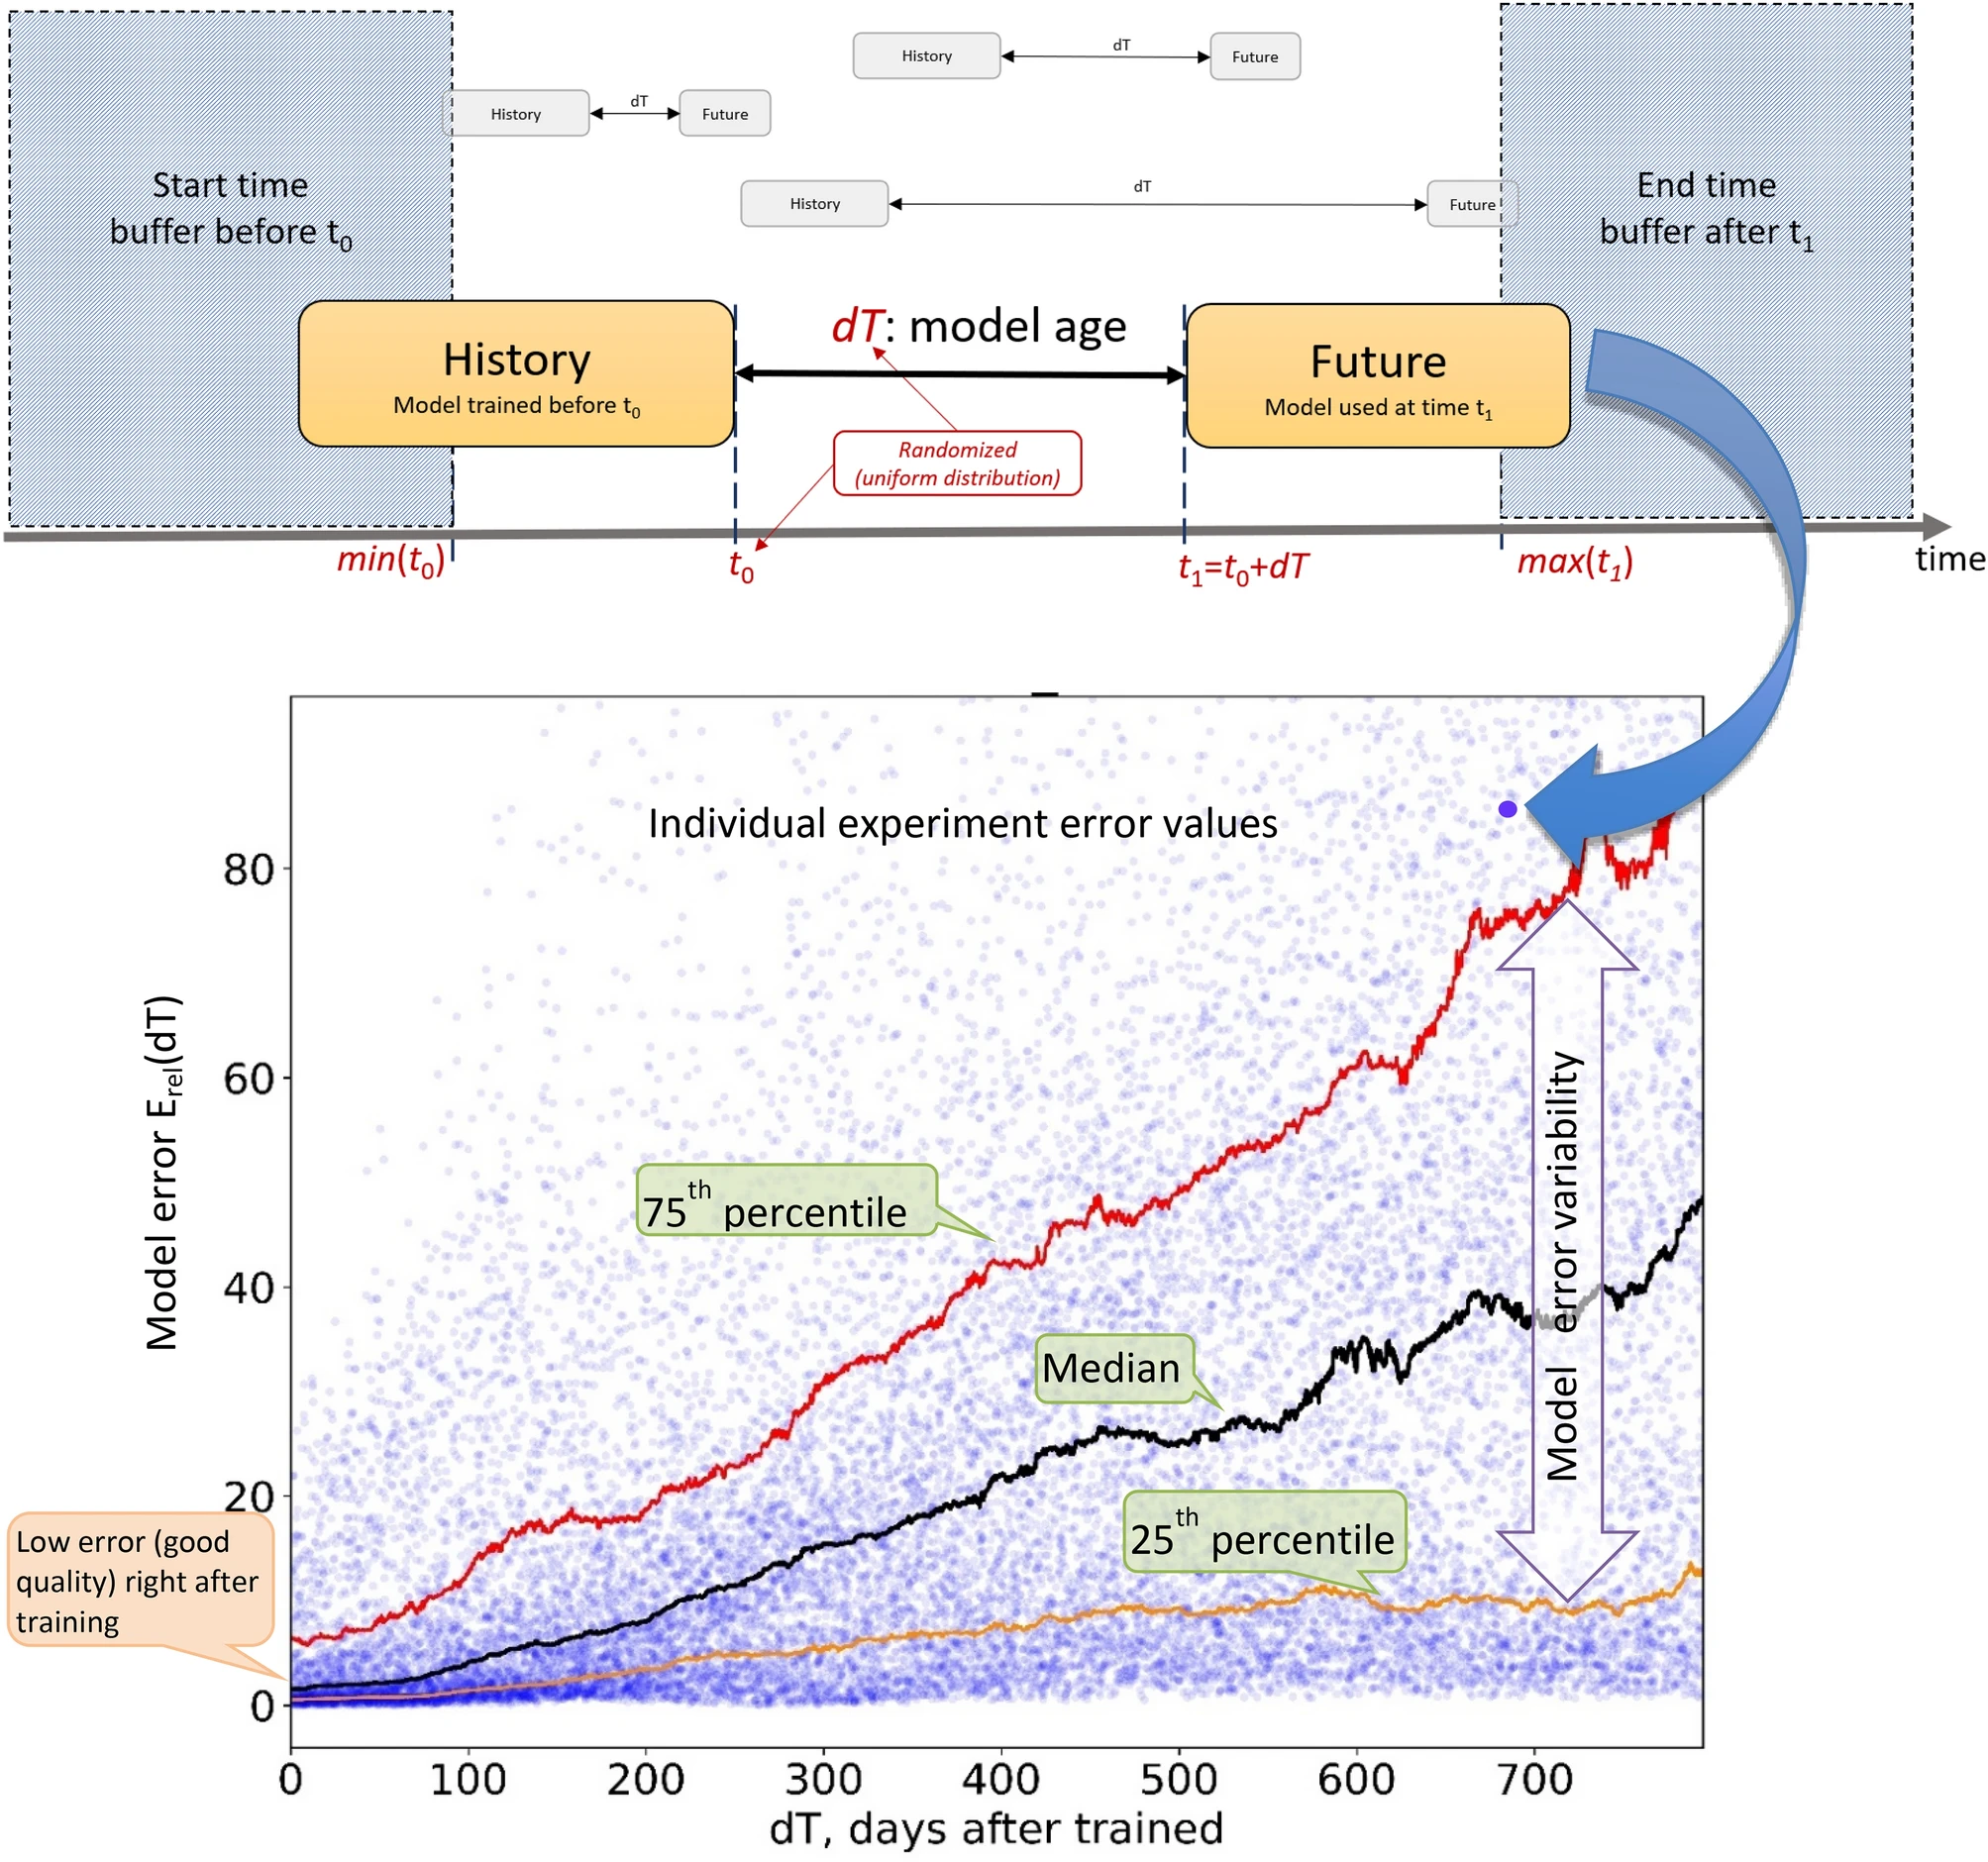
\includegraphics[width=.4\textwidth]{./figs/temporal/41598_2022_15245_Fig2_HTML.png}%
    
    \tiny See. \cite{vela2022temporal}
    
\end{frame}


\begin{frame}{Perspective : Foundation models ?}
    \centering
    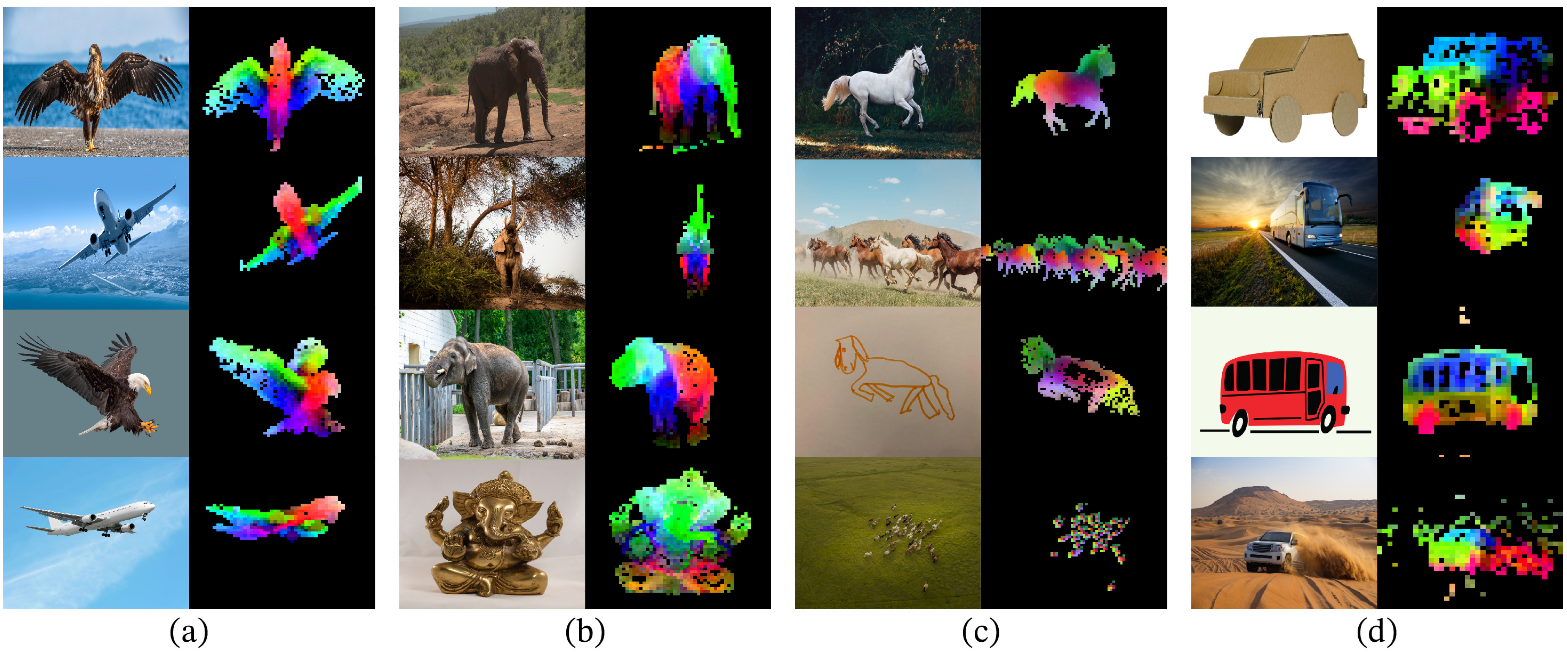
\includegraphics[width=.7\textwidth]{./figs/dinov2_pca.png}%
    
    \tiny See. \cite{oquab2023dinov2}
\end{frame}

\begin{frame}{Perspective : Foundation models ?}
    \centering
    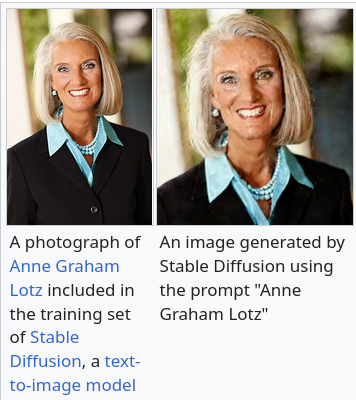
\includegraphics[width=.3\textwidth]{./figs/stable-diffusion.png}%
\end{frame}

\begin{frame}{Perspective : Foundation models ?}
    \centering
    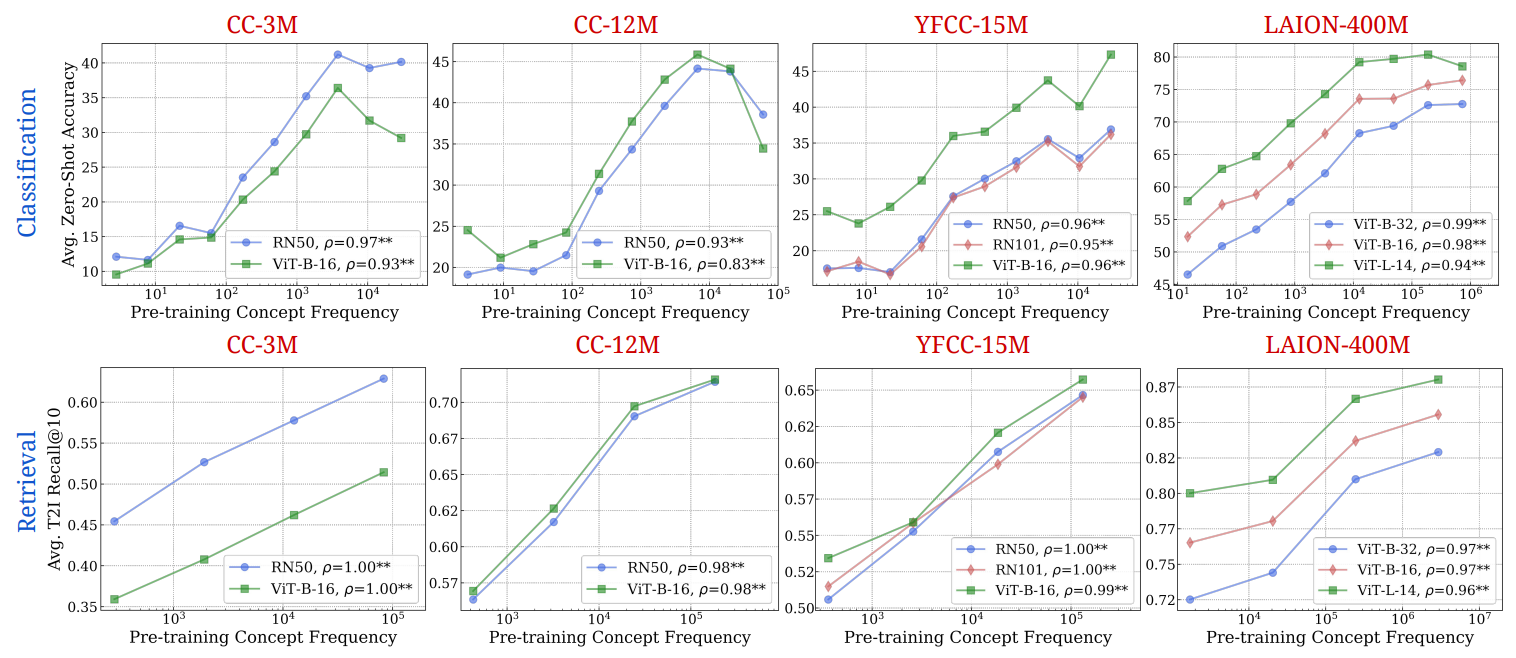
\includegraphics[width=.8\textwidth]{./figs/no_zero_shot.png}%
    
    \tiny See. \cite{udandarao2024no}
\end{frame}

\begin{frame}{Usefull ressources}

\begin{itemize}
    \item \texttt{scikit-learn} docs !
\end{itemize}
\end{frame}

\begin{frame}[plain]
    \Huge{\textbf{Thanks for you attention !}}
    
    \vfill
    
    \LARGE{\textbf{Let's practice !}}
\end{frame}

\appendix
\begin{frame}[allowframebreaks]{References}
\setbeamertemplate{bibliography item}{}
    {\footnotesize \printbibliography[heading=none]}
\end{frame}


\end{document}
